\documentclass[final]{article}

% if you need to pass options to natbib, use, e.g.:
% \PassOptionsToPackage{numbers, compress}{natbib}
% before loading nips_2017
%
% to avoid loading the natbib package, add option nonatbib:
% \usepackage[nonatbib]{nips_2017}

\PassOptionsToPackage{compress,authoryear,round}{natbib}
\usepackage{nips_2017}

% to compile a camera-ready version, add the [final] option, e.g.:
% \usepackage[final]{nips_2017}

\usepackage[utf8]{inputenc} % allow utf-8 input
\usepackage[T1]{fontenc}    % use 8-bit T1 fonts
\usepackage{hyperref}       % hyperlinks
\hypersetup{colorlinks=true,linkcolor=black,citecolor=black,filecolor=black,urlcolor=black,
            plainpages=false,pdfpagelabels,breaklinks=true,
  pdftitle    = {Brain Tumor Segmentation with Random Forest and U-Net},
  pdfsubject  = {},
  pdfauthor   = {Shuhan Xiao and Alexander Kugele},
  pdfkeywords = {} ,
  pdfcreator  = {pdflatex},
  pdfproducer = {}
}
\usepackage{url}            % simple URL typesetting
\usepackage{booktabs}       % professional-quality tables
\usepackage{amsfonts}       % blackboard math symbols
\usepackage{nicefrac}       % compact symbols for 1/2, etc.
\usepackage{microtype}      % microtypography

\makeatletter
\providecommand*{\input@path}{}
\g@addto@macro\input@path{{fig/}{../figures/}}
\makeatother

\usepackage{graphicx}
\graphicspath{{fig/}{../figures/}}

\usepackage{siunitx}
\usepackage{enumitem}
\usepackage{cleveref}

\title{Brain Tumor Segmentation with Random Forest and U-Net}

\author{
  Shuhan Xiao \\
  Heidelberg University \\
  \href{mailto:shuhan.xiao@stud.uni-heidelberg.de}{shuhan.xiao@stud.uni-heidelberg.de}\\
  \And
  Alexander Kugele \\
  Heidelberg University \\
  \href{mailto:a.kugele@stud.uni-heidelberg.de}{a.kugele@stud.uni-heidelberg.de}\\
}

\begin{document}

\maketitle

\begin{abstract}
.
\end{abstract}

\section{The Dataset}

\subsection{General Information}
Image segmentation is primarily done in two ways: Either designing an algorithm
from first principles or using available data to train an algorithm. As for
this challenge, designing an algorithm without data is very difficult, the
method of choice is training an algorithm from data. For the Multimodal Brain
Tumor Image Segmentation Benchmark \citep{BRATS} in 2015, 3D MR tumor scans
where collected from the BRATS 2012 and BRATS 2013 challenge and from the NIH
Cancer Imaging Archive (TCIA). In total, data for 55 low-grade glioma patients
and 220 high-grade glioma patients is provided. The data is a 16-bit 3D scan of
shape (depth=155, height=240, width=240), where all datasets have been aligned
to the same anatomical template and interpolated to \SI{1}{\mm^3} voxel
resolution. For each patient, four scan types are available: T1, T1c, T2 and
Flair. In the case of the BRATS data, the labels are from expert annotations of
one to four raters. The TCIA data labels were obtained by fusing the results of
multiple segmentation algorithms from the BRATS 2012 and BRATS 2013 challenge
and reviewed by expert raters.\\
Four classes are predefined:
\begin{enumerate}[label=\arabic*),topsep=0pt]
  \setcounter{enumi}{-1}
\item background
\item necrosis
\item edema
\item non-enhancing tumor
\item enhancing tumor
\end{enumerate}
Each 3D image for each scan type is saved in a seperate \verb+.mha+ file. The
average size per file is about \SI{2.2}{MB}, leading to approximately
$\SI{2.2}{MB}\cdot 275 \cdot 4 = \SI{2420}{MB}$ of compressed data.
Uncompressed, the data size increases to over \SI{100}{GB}. In
\cref{fig:dataex}, examples for LGG and HGG and the different scan types are
shown.

\begin{figure}
\centering
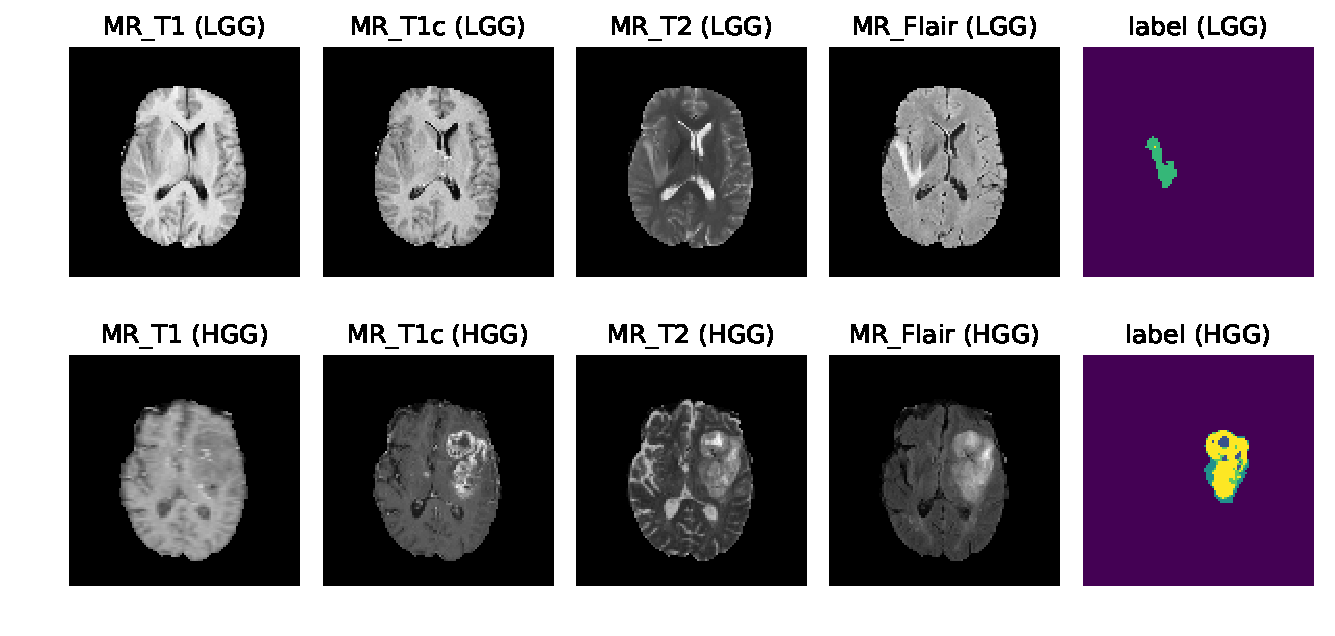
\includegraphics[width=0.99\linewidth]{scan_types_both}
\caption{Dataset examples. }
\label{fig:dataex}
\end{figure}

\subsection{Utilizing the Dataset}
The given images are sliced 3D scans. As we want to do segmentation in two
dimensions, we just take each slice as a separate input image. In total, this
are $155\cdot275\cdot4 = 170500$ input images. This full dataset proved too be
to large to use it for training. After trying out multiple subsets, it was
decided to use only the LGG part of the dataset and to sort out images where
the tumor to background ratio is less than $0.1\%$. This dataset only takes
\SI{110}{MB} compressed on disk. We split this dataset of 3315 images further
up into a training set of 2652 images ($80\%$) and a test set of 663 images.
This dataset is used for both the random forest and the U-Net. The classes are
reduced from five to two: background and tumor. Loading 10 images in the memory
of the GPU for training takes about \SI{3}{GB}. For the random forest, using
1000 images at once takes about \SI{30}{GB} of RAM.

\section{Random Forest}
The random forest is a set of decision trees, where each tree is fitted to a
random subset of the data and predictions are made by taking averages over the
predictions of individual trees. It 

\subsection{Features}
A random forest classifies each pixel separately. Therefore, using only the
pixel intensities would only give a good classification if the tumor can be
identified on a single-pixel level. To include information about the local
structure, multiple features are defined, such that each input pixel is an
N-dimensional vector.\\ The features we chose for this task are:
\begin{enumerate}
\item Gaussian filter
\begin{itemize}
\item Convolution with a Gaussian kernel
\item Smoothes the image
\end{itemize}
\item Laplacian of Gaussian (LoG) filter
\begin{itemize}
\item Convolution with the Laplacian of a Gaussian kernel
\item highlights edges (edges are 0)
\end{itemize}
\item Gaussian gradient magnitude filter
\begin{itemize}
\item Convolution with the gradient of a Gaussian kernel
\item highlights edges (edges are extrema)
\end{itemize}
\item Eigenvalues of the Hessian matrix
\begin{itemize}
\item determines the surface concavity
\end{itemize}
\item Eigenvalues of the structure tensor
\begin{itemize}
\item Summarizes gradient direction
\end{itemize}
\item Equalized histogram
\begin{itemize}
\item Enhances contrast
\end{itemize}
\end{enumerate}

Except the equalized histogram, they all share the tuneable kernel width
$\sigma$, which is set to $\{0.3, 0.7, 1., 3.5\}$. In total, $N=29$ filters are
used. In \cref{fig:features}, the features are shown for one example image of
the dataset for $\sigma = 0.3$. The tumor region in the bottom left can be
clearly identified for the Gaussian (bright), Laplacian of Gaussian (dark) and
the equalized histogram (bright). However, for other examples the tumor is also
pronounced in the other features.

In principle one could also utilize the different scan types as features.
However, the dataset is already very big and therefore it was decided to not
take the other scan types as features. This also allows for a fair comparison
between the random forest and the U-Net, as they are then trained with the same
dataset.

\begin{figure}
\centering
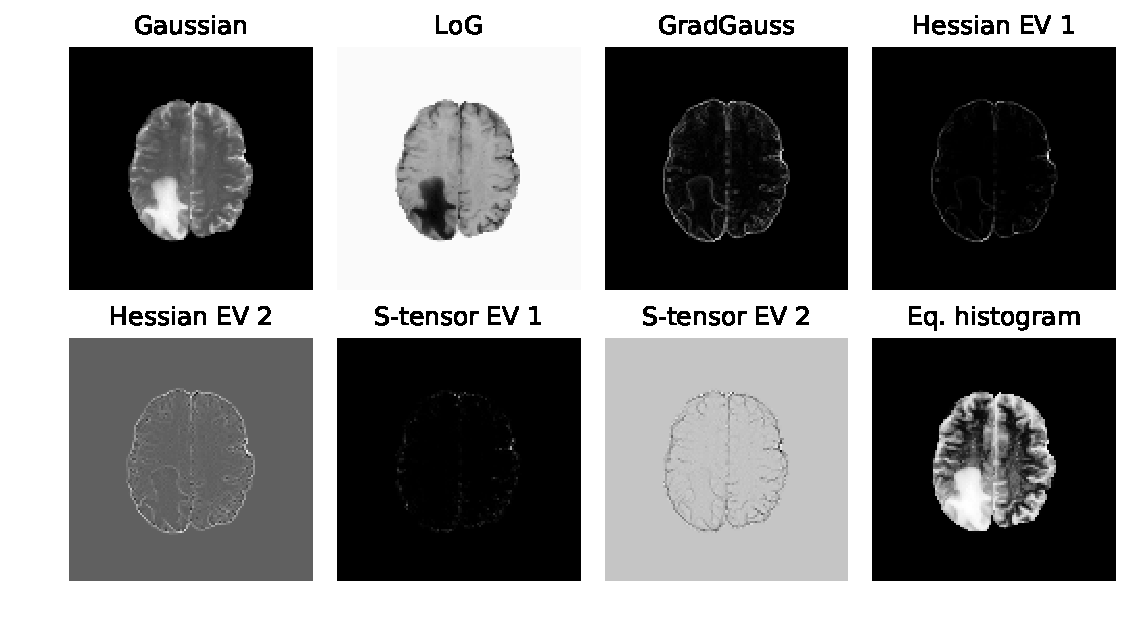
\includegraphics[width=0.99\textwidth]{features}
\caption{Features for the random forest. }
\label{fig:features}
\end{figure}

\bibliographystyle{plainnat}
\bibliography{../biblio}\vspace{0.75in}

\end{document}
